% ---
\chapter{INTRODUÇÃO}
% ---

%A formatação das referências bibliográficas conforme as regras da ABNT são um dos principais objetivos do \abnTeX. Consulte os manuais \citeonline{abntex2cite} e \citeonline{abntex2cite-alf} para obter informações sobre como utilizar as referências bibliográficas.
Quando a demanda por vagas de estacionamento aumentam demasiadamente, inevitavelmente se estabelece um reconhecido problema de congestionamento. Atualmente, é comum situações em que, por exemplo, nos campus universitários e regiões próximas aos centros das grandes cidades, a capacidade dos estacionamentos se esgotem facilmente. Geralmente dimensiona-se o número de vagas alocadas para estacionamentos no plano diretor das instituições públicas ou privadas. Estas vagas podem ser, à princípio, suficientes para atender a demanda de estacionamento dos veículos dos professores, funcionários, estudantes e visitantes no
anos iniciais. Porém, a previsão de crescimento do número de usuários, pode ser, por algum motivo, subestimada. Nas situações em que a demanda pelo estacionamento continua a crescer, o espaço reservado para acomodação dos veículos torna-se limitado. Outra situação a ser considerada é a de que 
alguma área livre do campus, geralmente seja utilizada na construção de novas salas de aula, escritórios e laboratórios, ou seja, as infra-estruturas que são consideradas mais importantes.
Em vista destas situações,  recorrem-se às estratégias de gestão e a Sistemas de Transporte Inteligentes (Intelligent
Transportation Systems, ITS) para lidar com o problema de congestionamento do estacionamento, em vez da capacidade de 
expansão.
Pode-se argumentar que o acesso ao estacionamento é um fator que determina se e como os usuários chegam aos
campus das universidades e institutos federais. Normalmente, nestes estabelecimentos, a maioria dos usuários possuem seu próprio horário de trabalho ou estudo e a demanda de estacionamento é relativamente inelástica. 
Algumas alternativas para mitigar o problema do congestionamento nos estacionamentos podem ser antipáticas aos usuários, dentre estas, pode-se citar a
administração do estacionamento por meio de uma combinação de cobrança pelo direito de estacionar ou fornecer modos de transporte alternativos. Outra abordagem admitida para resolver o problema de congestionamento do estacionamento do campus é resolver o problema pelo lado da oferta; isto é, implementar políticas para melhor controle do uso do estacionamento e usar o ITS para
tornar o uso do estacionamento mais eficiente. A dificuldade de encontrar uma vaga de estacionamento não apenas contribui para o congestionamento do tráfego dentro da repartição ou estabelecimento, mas também nas ruas circundantes, ao procurar uma vaga vazia para estacionar, os veículos em circulação utilizam a marcha lenta e podem aumentar as emissões de gases nocivos resultantes da queima de combustível, afetando negativamente a saúde da comunidade e prejudicando o meio ambiente. Deve-se
aumentar a conscientização dos tomadores de decisão das instituições públicas e privadas sobre a importância de evitar o congestionamento dos estacionamentos e
aumentar a compreensão dos impactos dos estacionamentos no meio ambiente e na saúde da comunidade.
O ideal a ser alcançado deve, preferencialmente, contar com projetos de estacionamentos que consigam evitar seu congestionamento.


%O software de back-end é construído sob o guarda-chuva de Ruby nos trilhos. O Ruby on Rails é uma estrutura em vez de uma peça de tecnologia. Seu objetivo é facilitar a desenvolvimento de aplicativos da web, tornando a integração de tecnologias da Web díspares o mais transparente possível, para que o cliente, o servidor e o banco de dados possam ser desenvolvidos e implantado em conjunto de forma simples, eficiente e limpa. A pilha de tecnologia de back-end consiste em plat software de formulário e software de aplicação. Uma visão geral do principais componentes a seguir: Tecnologia da plataforma: Heroku: O Heroku é uma plataforma em nuvem para hospedagem de aplicativos baseados na Web que oferece alta escalabilidade arquitetura e integração simples de software de terceiros com vários provedores de serviços em nuvem. Postgresql: Postgresql fornece banco de dados relacional Software e é usado para armazenar todos os aplicativos relacionados a aplicativos. dados. NGNX: este é um HTTP de alto desempenho (Hyper protocolo de transferência de texto).Unicórnio: servidor Web baseado em  Ruby que age como uma cola entre NGNX e Ruby on Rails (ou outros aplicativos baseados em rack Aplicativos da web)


\section{Tema}
 Alguns campus do IFRN, notadamente, o de Natal Central, vêm enfrentando situações semelhantes as descritas anteriormente. No intuito de organizar e registrar o ingresso de veículos as suas  dependências, este trabalho de conclusão de curso propõe o desenvolvimento de um sistema web para controle dos veículos e acesso ao estacionamento do Instituto Federal de Educação, Ciência e Tecnologia Rio Grande do Norte - IFRN, visando controlar os veículos que podem ter acesso ao estacionamento da instituição.  
 
 \section{Objetivo Geral}\label{sec:objetivos}
 %\addcontentsline{toc}{section}{Objetivos}
 %\lipsum[36]
 %\subsection{}
 A proposta deste trabalho de conclusão de curso consiste em desenvolver um sistema web administrativo completo, com autenticação, para controle de veículos e acesso aos estacionamentos dos campi do IFRN.
 \section{Objetivos Específicos}
 \begin{itemize}
 	\item Utilizar a estrutura Ruby on Rails (RoR) \cite{hartl2011ruby} para desenvolvimento do sistema web.
 	\item Utilizar o banco de dados  PostgreSQL.
 	\item Apresentar um caso de uso com o sistema elaborado.
 \end{itemize}
 
 \section{Delimitação do Problema} 
Apresentar um sistema web administrativo completo, com autenticação, para controle de veículos e acesso aos estacionamentos dos campi do IFRN.
%-
\section{Motivações e Justificativas}
%-
Tendo em vista que a quantidade de vagas no estacionamento do campus Natal Central do IFRN é limitado e que a quantidade de veículos ocupantes está aumentando gradativamente, é necessário controlar o acesso dos veículos que realmente possuem prerrogativa para sua utilização, tais como aqueles pertencentes a servidores do instituto e visitantes. Além da quantidade, o processo para cadastro de um funcionário, que possua um veículo, é bastante burocrático, exigindo a comunicação entre um certo número de funcionários, por exemplo, diretor e  departamento de segurança, para autorização do registro, dificultando a aquisição do adesivo que identifica um veículo habilitado. A abordagem de uma solução para o problema de congestionamento e dificuldades para organização e liberação de autorizações, culmina na necessidade do desenvolvimento de um sistema que gerencie esse, e, possivelmente, outros estacionamentos. Esta é uma grande oportunidade de aplicar os conceitos apresentados nas diversas disciplinas estudadas no curso técnico de informática para internet, ofertado pelo IFRN, na modalidade de ensino à distância. Particularmente, no presente trabalho, optou-se por desenvolver o referido sistema utilizando a(o) estrutura/framework Ruby On Rails (RoR) e banco de dados PostgreSQL. Nesse sentido, o desafio que se apresentou é de certa maneira complexo e instigante, pois tratam-se de ferramentas elaboradas e que exigem considerável nível de conhecimento para sua utilização adequada. 
%A estrutura Ruby on Rails (RoR) \cite{hartl2011ruby} é adotada para desenvolver o serviço da Web, pois permite ao designer organizar o aplicativo como uma coleção de casos de uso que podem ser reutilizados para tarefas semelhantes (\cite{faro1998storynet}. Além disso, o RoR é fornecido com uma linguagem poderosa, ou seja, Ruby, que facilita a implementação de: a) as regras difusas que abordam a mobilidade do usuário e auxiliam suas decisões e b) aprocedimentos para acessar a camada de metadados que integram os diferentes bancos de dados. Outros dois idiomas também podem ser usados no RoR para facilitar aimplementação de aplicativos LBS: a) scripts Java para trocar informações móveis georreferenciadas no Google Maps; b) JQueryMobile (Bai, 2011) para transmitir essas informações em um formato amigável que pode ser visualizado, sem qualquer modificação, em PCs, tablets e celulares.

%Normalmente não há problemas em usar caracteres acentuados em arquivos bibliográficos (\texttt{*.bib}). Porém, como as regras da ABNT fazem uso quase abusivo da conversão para letras maiúsculas, é preciso observar o modo como se escreve os nomes dos autores. Na~\autoref{tabela-acentos} você encontra alguns exemplos das conversões mais importantes. Preste atenção especial para `ç' e `í' que devem estar envoltos em chaves. A regra geral é sempre usar a acentuação neste modo quando houver conversão para letras maiúsculas.

%\begin{table}[htbp]
%\caption{Tabela de conversão de acentuação.}
%\label{tabela-acentos}

%\begin{center}
%\begin{tabular}{ll}\hline\hline
%acento & \textsf{bibtex}\\
%à á ã & \verb+\`a+ \verb+\'a+ \verb+\~a+\\
%í & \verb+{\'\i}+\\
%ç & \verb+{\c c}+\\
%\hline\hline
%\end{tabular}
%\end{center}
%\end{table}


% ---
%\section{Precisa de ajuda?}
% ---

%Consulte a FAQ com perguntas frequentes e comuns no portal do \abnTeX: \url{https://code.google.com/p/abntex2/wiki/FAQ}. Inscreva-se no grupo de usuários \LaTeX: \url{http://groups.google.com/group/latex-br}, tire suas dúvidas e ajude outros usuários.

\section{Método de Trabalho}
\label{MétodoTrabalho}
O presente trabalho de conclusão de curso utilizou as funcionalidades do Rails Admin, 
um mecanismo, disponibilizado na internet, que fornece uma interface fácil de usar para gerenciamento de dados \cite{adminGitHub2018}. Adicionalmente, utilizou-se como Sistema de Gerenciamento de Banco de Dados (SGBD), o PostgreSQL. Identificou-se como uma necessidades muito importante para a comunidade acadêmica do IFRN, propor soluções para o problema de desorganização do acesso dos usuários aos estacionamentos da instituição. Dessa forma, o presente trabalho propõe um meio de gerenciar de maneira simples os estacionamentos da instituição. 
Inicialmente, analisou-se as causas mais prováveis da má utilização dos estacionamentos. Pode-se citar, por exemplo, o acesso de pessoas não autorizadas, que não possuem vínculo com o IFRN.

Concomitantemente, estudou-se mais aprofundadamente a linguagem de programação Ruby, e a utilização da estrutura Ruby on Rails. Com essas ferramentas principais  implementou-se um sistema administrativo em conjunto com a base de dados. Além disso foram empregados
conhecimentos em HTML, CSS e Javascript. 
Para a criação da plataforma que irá gerenciar o estacionamento de veículos, foi utilizada \texttt{gems} específicas, que simplificam a criação de um sistema administrativo. Dessa forma, criou-se  os seguintes modelos: \texttt{estacionamento}, \texttt{veiculo}, \texttt{funcionario} e \texttt{vaga}. Os parâmetros de cada modelo, bem como suas relações e as \texttt{gems} utilizadas, serão descritas mais à frente.

\section{Organização do Trabalho}
Em sua organização, o presente trabalho possui capítulos apresentados da seguinte maneira:
\begin{itemize}
	\item Desenvolvimento:\\
	No segundo capítulo são apresentadas as ferramentas tecnológicas empregadas na construção do software e os requisitos funcionais e não-funcionais. Nessa oportunidade descrevem-se em  detalhes cada aplicação realizada. Mostram-se, adicionalmente, a maneira de integração com o banco de dados, diagramas para o entendimento do sistema criado, as categorias de usuários e as atribuições que esses tem acesso.  
	\item Avaliação:\\
	No terceiro capítulo, caracteriza-se a verificação do sistema e apresentam-se os resultados de seu funcionamento. 
	\item Conclusão:\\
	No quarto e último capítulo, argumenta-se conclusivamente a respeito do software construído. Igualmente, pondera-se sobre possíveis melhorias em trabalhos futuros.
\end{itemize}

\section{Equipe e Infraestrutura}

O presente TCC foi concebido e escrito individualmente pelo autor que contou com uma infraestrutura simples constituída por seu notebook pessoal $idepad^{S145}$, core $\texttt{i5}$, marca lenovo e acesso à intenet.



\section{Cronograma de Acompanhamento}
\label{CronoAcomp}
O cronograma do trabalho encontra-se na Tabela \ref{tab-cronograma}, onde as etapas são:

\begin{itemize}
	\item 1º) \textbf{Iniciação:} Definição do problema; Apresentação de proposta de solução com os requisitos funcionais e suplementares; Levantamento bibliográfico;  Feedback do orientador.
	\item 2º) \textbf{Elaboração:} Protótipo de Arquitetura; Análise inicial; Estudo e utilização da \texttt{gem} 'rails\_admin'; \texttt{gem} 'Devise'; Estudo aprofundado de Relacionamentos em Ruby; Estudo detalhado em gerenciamento de banco de dados utilizando PostgreSQL;  Feedback do orientador.
	\item 3º) \textbf{Construção:}  Implementação e verificação dos requisitos que foram definidos; Feedback do orientador.
	\item 4º) \textbf{Transição:} Conclusão do protótipo e documentação; Feedback do orientador.
	%\item 5º) Relatório/síntese dos resultados.
\end{itemize}

\begin{table}[h!]\begin{center}
		\caption{Cronograma}\label{tab-cronograma}
		\begin{tabular*}{\textwidth}{@{\extracolsep{\fill}} c c c c c c c c c c c c}
			\toprule
			& Etapa & ago. & set. & out. & nov. & dez. & jan. (2020). & fev. (2020) & mar. (2020) &\\
			\midrule
			&   1   &   x  &   x  &   x   &      &      &      &     \\
			&   2   &   x  &   x  &   x  &   x   &   x   &   x   &  x   &      &      &\\
			&   3   &      &   x   &   x  &   x  &   x  &   x  &   x   & x & \\
			&   4   &      &      &      &      &      &   x  &   x  &  x & \\
			
			\bottomrule                             
		\end{tabular*}
\end{center}\end{table}


\section{Marcos do Projeto}

A Figura \ref{marcos}  mostra os marcos significativos do
projeto, indicando os artefatos que serão entregues.

\begin{table}[h]
	\centering
	\caption{Marcos do Projeto}
	\label{marcos}
	\resizebox{\textwidth}{!}{
\begin{ganttchart}{1}{16}
	\gantttitle{2019-2020}{16} \\
	\gantttitlelist{1,...,16}{1} \\
	\ganttgroup{José Victor G. F.}{8}{15} \\
	\ganttbar{Iniciação}{8}{10} \\
	\ganttlinkedbar{Elaboração}{8}{12} \ganttnewline
	\ganttmilestone{1º Marco: Primeiro
		Release
}{12} \ganttnewline
	\ganttbar{Transição}{8}{15}\ganttnewline
	\ganttmilestone{2º Marco: Release
		Final}{15} \ganttnewline
	\ganttlink{elem2}{elem3}
	\ganttlink{elem3}{elem4}
	\ganttlink{elem4}{elem5}
\end{ganttchart}
}
\hrulefill
\end{table}

\section{Gerência de Riscos}
Para o desenvolvimento da plataforma de gerenciamento do presente trabalho buscou-se controlar, na medida do possível, alguns fatores. 
As Fig. \ref{figura:riscos1} e \ref{figura:riscos2} mostram, respectivamente, os riscos externos e internos presumidos. 


\begin{figure}[h]
	\caption{Riscos Externos.}
	
	\centering % para centralizarmos a figura
	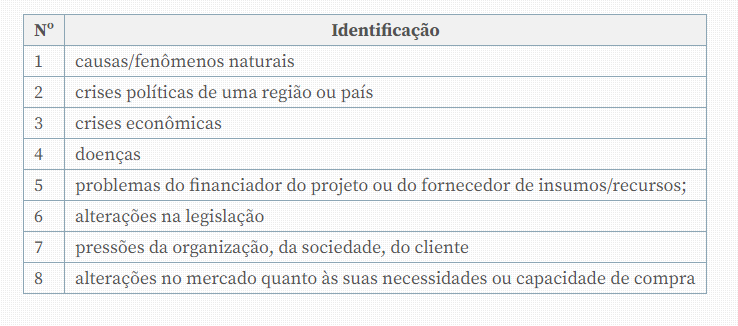
\includegraphics[scale=0.85]{Figs/riscos1.png} % leia abaixo
	\label{figura:riscos1}
\end{figure}

\begin{figure}[h]
	\caption{Riscos Internos.}
	
	\centering % para centralizarmos a figura
	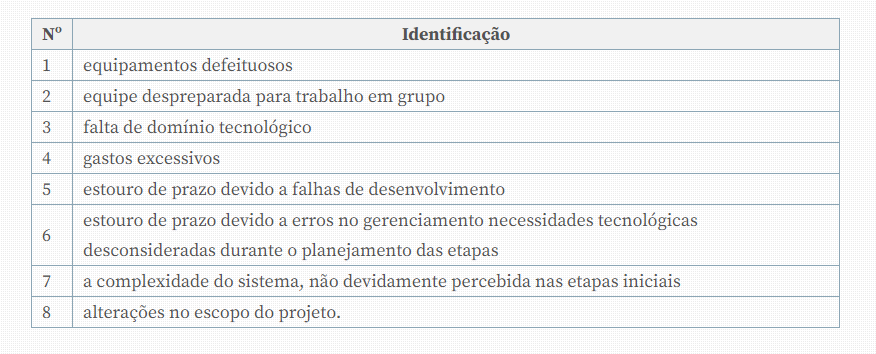
\includegraphics[scale=0.72]{Figs/riscos2.png} % leia abaixo
	\label{figura:riscos2}
\end{figure}

%Deve-se destacar que a pressão da organização (IFRN), no atraso da definição dos temas de projetos e na ausência de melhor orientação para execução dos trabalhos, além da falta de domínio tecnológico, têm contribuído significativamente para o atraso da entrega do produto. Nessa perspectiva o planejamento de resposta aos riscos levou em consideração a possibilidade de continuidade do trabalho no próximo semestre conforme dialogado com o prof. orientador do TCC.

\section{Qualidade do Sistema}

 O presente projeto levou em consideração o desenvolvimento de um software de qualidade primando por sua confiabilidade e usabilidade. Atualmente, trabalha-se para que a plataforma de gerenciamento execute completamente suas funcionalidades. O emprego das \texttt{gems} mencionadas na seção \ref{CronoAcomp} proporciona ao sistema fácil manutenção, mantendo a integridade dos dados e evitando possíveis falhas. A referência básica que levou-se em consideração foi a ISO/IEC 9126(NBR13596) que pode ser consultada em \cite{qualidadeSoftware2008}. Para se garantir a qualidade do produto durante seu desenvolvimento seguiu-se um conjunto de métodos e técnicas cuja implementação têm acontecido ao longo das etapas. As atividades de validação, verificação e testes contarão com revisões de software e é apresentada na seção 
\ref{testesSoft} %Atualmente trabalha-se para se identificar as causas de algumas falhas que o primeiro protótipo do sistema apresenta e corrigi-lo.
%\section{Glossário}